% Options for packages loaded elsewhere
\PassOptionsToPackage{unicode}{hyperref}
\PassOptionsToPackage{hyphens}{url}
\PassOptionsToPackage{dvipsnames,svgnames,x11names}{xcolor}
%
\documentclass[
  11pt,
  letterpaper,
]{article}
\usepackage{amsmath,amssymb}
\usepackage{iftex}
\ifPDFTeX
  \usepackage[T1]{fontenc}
  \usepackage[utf8]{inputenc}
  \usepackage{textcomp} % provide euro and other symbols
\else % if luatex or xetex
  \usepackage{unicode-math} % this also loads fontspec
  \defaultfontfeatures{Scale=MatchLowercase}
  \defaultfontfeatures[\rmfamily]{Ligatures=TeX,Scale=1}
\fi
\usepackage{lmodern}
\ifPDFTeX\else
  % xetex/luatex font selection
  \setmainfont[]{Latin Modern Roman}
  \setsansfont[]{DejaVu Sans}
  \setmonofont[]{DejaVu Sans Mono}
\fi
% Use upquote if available, for straight quotes in verbatim environments
\IfFileExists{upquote.sty}{\usepackage{upquote}}{}
\IfFileExists{microtype.sty}{% use microtype if available
  \usepackage[]{microtype}
  \UseMicrotypeSet[protrusion]{basicmath} % disable protrusion for tt fonts
}{}
\makeatletter
\@ifundefined{KOMAClassName}{% if non-KOMA class
  \IfFileExists{parskip.sty}{%
    \usepackage{parskip}
  }{% else
    \setlength{\parindent}{0pt}
    \setlength{\parskip}{6pt plus 2pt minus 1pt}}
}{% if KOMA class
  \KOMAoptions{parskip=half}}
\makeatother
\usepackage{xcolor}
\usepackage[top=2.1cm,bottom=2.1cm,left=2.2cm,right=2.2cm]{geometry}
\usepackage{color}
\usepackage{fancyvrb}
\newcommand{\VerbBar}{|}
\newcommand{\VERB}{\Verb[commandchars=\\\{\}]}
\DefineVerbatimEnvironment{Highlighting}{Verbatim}{commandchars=\\\{\}}
% Add ',fontsize=\small' for more characters per line
\newenvironment{Shaded}{}{}
\newcommand{\AlertTok}[1]{\textcolor[rgb]{1.00,0.00,0.00}{\textbf{#1}}}
\newcommand{\AnnotationTok}[1]{\textcolor[rgb]{0.38,0.63,0.69}{\textbf{\textit{#1}}}}
\newcommand{\AttributeTok}[1]{\textcolor[rgb]{0.49,0.56,0.16}{#1}}
\newcommand{\BaseNTok}[1]{\textcolor[rgb]{0.25,0.63,0.44}{#1}}
\newcommand{\BuiltInTok}[1]{\textcolor[rgb]{0.00,0.50,0.00}{#1}}
\newcommand{\CharTok}[1]{\textcolor[rgb]{0.25,0.44,0.63}{#1}}
\newcommand{\CommentTok}[1]{\textcolor[rgb]{0.38,0.63,0.69}{\textit{#1}}}
\newcommand{\CommentVarTok}[1]{\textcolor[rgb]{0.38,0.63,0.69}{\textbf{\textit{#1}}}}
\newcommand{\ConstantTok}[1]{\textcolor[rgb]{0.53,0.00,0.00}{#1}}
\newcommand{\ControlFlowTok}[1]{\textcolor[rgb]{0.00,0.44,0.13}{\textbf{#1}}}
\newcommand{\DataTypeTok}[1]{\textcolor[rgb]{0.56,0.13,0.00}{#1}}
\newcommand{\DecValTok}[1]{\textcolor[rgb]{0.25,0.63,0.44}{#1}}
\newcommand{\DocumentationTok}[1]{\textcolor[rgb]{0.73,0.13,0.13}{\textit{#1}}}
\newcommand{\ErrorTok}[1]{\textcolor[rgb]{1.00,0.00,0.00}{\textbf{#1}}}
\newcommand{\ExtensionTok}[1]{#1}
\newcommand{\FloatTok}[1]{\textcolor[rgb]{0.25,0.63,0.44}{#1}}
\newcommand{\FunctionTok}[1]{\textcolor[rgb]{0.02,0.16,0.49}{#1}}
\newcommand{\ImportTok}[1]{\textcolor[rgb]{0.00,0.50,0.00}{\textbf{#1}}}
\newcommand{\InformationTok}[1]{\textcolor[rgb]{0.38,0.63,0.69}{\textbf{\textit{#1}}}}
\newcommand{\KeywordTok}[1]{\textcolor[rgb]{0.00,0.44,0.13}{\textbf{#1}}}
\newcommand{\NormalTok}[1]{#1}
\newcommand{\OperatorTok}[1]{\textcolor[rgb]{0.40,0.40,0.40}{#1}}
\newcommand{\OtherTok}[1]{\textcolor[rgb]{0.00,0.44,0.13}{#1}}
\newcommand{\PreprocessorTok}[1]{\textcolor[rgb]{0.74,0.48,0.00}{#1}}
\newcommand{\RegionMarkerTok}[1]{#1}
\newcommand{\SpecialCharTok}[1]{\textcolor[rgb]{0.25,0.44,0.63}{#1}}
\newcommand{\SpecialStringTok}[1]{\textcolor[rgb]{0.73,0.40,0.53}{#1}}
\newcommand{\StringTok}[1]{\textcolor[rgb]{0.25,0.44,0.63}{#1}}
\newcommand{\VariableTok}[1]{\textcolor[rgb]{0.10,0.09,0.49}{#1}}
\newcommand{\VerbatimStringTok}[1]{\textcolor[rgb]{0.25,0.44,0.63}{#1}}
\newcommand{\WarningTok}[1]{\textcolor[rgb]{0.38,0.63,0.69}{\textbf{\textit{#1}}}}
\usepackage{longtable,booktabs,array}
\usepackage{calc} % for calculating minipage widths
% Correct order of tables after \paragraph or \subparagraph
\usepackage{etoolbox}
\makeatletter
\patchcmd\longtable{\par}{\if@noskipsec\mbox{}\fi\par}{}{}
\makeatother
% Allow footnotes in longtable head/foot
\IfFileExists{footnotehyper.sty}{\usepackage{footnotehyper}}{\usepackage{footnote}}
\makesavenoteenv{longtable}
\usepackage{graphicx}
\makeatletter
\def\maxwidth{\ifdim\Gin@nat@width>\linewidth\linewidth\else\Gin@nat@width\fi}
\def\maxheight{\ifdim\Gin@nat@height>\textheight\textheight\else\Gin@nat@height\fi}
\makeatother
% Scale images if necessary, so that they will not overflow the page
% margins by default, and it is still possible to overwrite the defaults
% using explicit options in \includegraphics[width, height, ...]{}
\setkeys{Gin}{width=\maxwidth,height=\maxheight,keepaspectratio}
% Set default figure placement to htbp
\makeatletter
\def\fps@figure{htbp}
\makeatother
\setlength{\emergencystretch}{3em} % prevent overfull lines
\providecommand{\tightlist}{%
  \setlength{\itemsep}{0pt}\setlength{\parskip}{0pt}}
\setcounter{secnumdepth}{-\maxdimen} % remove section numbering
\ifLuaTeX
\usepackage[bidi=basic]{babel}
\else
\usepackage[bidi=default]{babel}
\fi
\babelprovide[main,import]{spanish}
\ifPDFTeX
\else
\babelfont{rm}[]{Latin Modern Roman}
\fi
% get rid of language-specific shorthands (see #6817):
\let\LanguageShortHands\languageshorthands
\def\languageshorthands#1{}
\usepackage{fancyhdr}
\usepackage{xurl}
\usepackage{etoolbox}
\usepackage{needspace}
\usepackage{float}
\usepackage{caption}
\pagestyle{fancy}
\fancyhf{}
\fancyhead[L]{\small Rendimiento académico}
\fancyhead[R]{\small Regresión lineal múltiple}
\fancyfoot[C]{\small\thepage}
\setlength{\headheight}{15pt}
\renewcommand{\headrulewidth}{0pt}
\renewcommand{\arraystretch}{1.16}
\setlength{\tabcolsep}{4.2pt}
\setlength{\parskip}{5pt}
\setlength{\parindent}{0pt}
\captionsetup{font=small,labelformat=empty,skip=5pt}
\floatplacement{figure}{H}
\AtBeginEnvironment{longtable}{\small}
\setlength{\emergencystretch}{3em}
\ifLuaTeX
  \usepackage{selnolig}  % disable illegal ligatures
\fi
\IfFileExists{bookmark.sty}{\usepackage{bookmark}}{\usepackage{hyperref}}
\IfFileExists{xurl.sty}{\usepackage{xurl}}{} % add URL line breaks if available
\urlstyle{same}
\hypersetup{
  pdftitle={Rendimiento académico mediante regresión lineal múltiple},
  pdfauthor={Frank Arlom Rico; Emily Daniela Hernandez; Jhoan Sebastian Ramirez Monsalve},
  pdflang={es},
  colorlinks=true,
  linkcolor={black},
  filecolor={Maroon},
  citecolor={Blue},
  urlcolor={black},
  pdfcreator={LaTeX via pandoc}}

\title{Rendimiento académico mediante regresión lineal múltiple}
\usepackage{etoolbox}
\makeatletter
\providecommand{\subtitle}[1]{% add subtitle to \maketitle
  \apptocmd{\@title}{\par {\large #1 \par}}{}{}
}
\makeatother
\subtitle{Análisis de una base simulada y evaluación de su capacidad
predictiva}
\author{Frank Arlom Rico \and Emily Daniela Hernandez \and Jhoan
Sebastian Ramirez Monsalve}
\date{24 de octubre de 2026}

\begin{document}
\thispagestyle{plain}
\begin{center}
{\Large Rendimiento académico mediante regresión lineal múltiple\par}
\vspace{4pt}
{\normalsize Análisis de una base simulada y evaluación de su capacidad predictiva\par}
\vspace{10pt}
{\normalsize\textbf{Integrantes}\par}
Frank Arlom Rico\\
Emily Daniela Hernandez\\
Jhoan Sebastian Ramirez Monsalve
\par\vspace{8pt}
{\small 24 de octubre de 2026\par}
\vspace{4pt}
{\small\textbf{Repositorio del proyecto}\par}
{\footnotesize\url{https://github.com/jhoanramirezm96/Trabajo_Regresion_Multiple}\par}
\end{center}
\vspace{3pt}


\hypertarget{suxedntesis-del-anuxe1lisis}{%
\subsection{Síntesis del análisis}\label{suxedntesis-del-anuxe1lisis}}

Se ajustó una regresión lineal múltiple para explicar el rendimiento
académico a partir de hábitos de estudio, asistencia, condiciones
psicosociales y otras características. El análisis utiliza 2.000
observaciones \textbf{simuladas con el script suministrado en la
actividad}. El modelo explica el 68,46 \% de la variación observada y
alcanza un RMSE de 0,304 puntos en una prueba de 400 registros que no
participaron en su entrenamiento. Las horas de estudio y la motivación
presentan asociaciones positivas. El estrés y las asignaturas reprobadas
presentan asociaciones negativas. El estrato no muestra evidencia
estadística suficiente de asociación lineal parcial en esta
especificación.

El ajuste es útil para el ejercicio. Su alcance es didáctico: las
relaciones principales fueron incorporadas al generar los datos. Además,
se encontraron horas negativas y una limitación de la regresión
ordinaria para respetar el rango de la nota. Por ello, los resultados no
permiten establecer causas ni formular conclusiones sobre una población
universitaria real.

\hypertarget{planteamiento-y-procedencia-de-los-datos}{%
\subsection{1 Planteamiento y procedencia de los
datos}\label{planteamiento-y-procedencia-de-los-datos}}

La pregunta de trabajo es: \textbf{¿cómo se relacionan las variables
incluidas en el material con el rendimiento académico y qué tan bien
permite predecirlo un modelo lineal múltiple?} Se busca estimar esas
asociaciones, interpretar sus coeficientes bajo control de las demás
variables y evaluar tanto los supuestos como el error fuera de muestra.

La revisión de los archivos mostró una diferencia que afecta el
desarrollo de la actividad. Aunque se llama
\texttt{dataset\_RegMultiple.xlsx}, el Excel contiene 90 registros y
tres columnas: \texttt{ID}, \texttt{Metodo} y \texttt{Puntaje}. No
contiene las variables del modelo propuesto. Por su parte,
\texttt{Dataset\_RegMultiple.R} genera una base de 2.000 registros con
15 variables de rendimiento académico. Se adoptó esta segunda fuente por
su correspondencia con la consigna y el ejemplo de regresión.

La base utilizada se reconstruyó en R 4.3.3 con \texttt{set.seed(123)} y
los generadores Mersenne-Twister, Inversion y Rejection. Se conservaron
las distribuciones, el orden de las operaciones y la ecuación del
archivo original. El error de exportación se resolvió usando el objeto
\texttt{datos}, que es el creado por el script; el original intentaba
exportar un objeto llamado \texttt{dataset}. La copia recibida no se
modificó.

El procedimiento se presenta como una \textbf{simulación académica}. La
actividad aborda un problema real, pero sus archivos no aportan una
muestra observacional de estudiantes. Esta diferencia determina cómo
deben leerse las conclusiones.

\newpage

\hypertarget{variables-y-revisiuxf3n-de-calidad}{%
\subsection{2 Variables y revisión de
calidad}\label{variables-y-revisiuxf3n-de-calidad}}

La variable respuesta es \texttt{rendimiento}, una nota limitada al
intervalo de 0 a 5. Se conservaron los diez predictores de la fórmula
del material. La siguiente tabla precisa su codificación y evita
confundir las unidades de los coeficientes.

\begin{longtable}[]{@{}
  >{\raggedright\arraybackslash}p{(\columnwidth - 2\tabcolsep) * \real{0.2700}}
  >{\raggedright\arraybackslash}p{(\columnwidth - 2\tabcolsep) * \real{0.7300}}@{}}
\toprule\noalign{}
\begin{minipage}[b]{\linewidth}\raggedright
Variable
\end{minipage} & \begin{minipage}[b]{\linewidth}\raggedright
Significado y tratamiento
\end{minipage} \\
\midrule\noalign{}
\endhead
\bottomrule\noalign{}
\endlastfoot
\texttt{rendimiento} & Nota simulada de 0 a 5. Respuesta
cuantitativa. \\
\texttt{horas\_estudio} & Cantidad de horas de estudio. El material no
especifica el período de referencia. \\
\texttt{asistencia} & Porcentaje de asistencia entre 70 y 100. Un
incremento de una unidad equivale a un punto porcentual. \\
\texttt{motivacion} & Puntuación simulada de 1 a 5, con decimales. Se
trata como cuantitativa. \\
\texttt{estres} & Puntuación simulada de 1 a 5, con decimales. Se trata
como cuantitativa. \\
\texttt{apoyo\_familiar} & Puntuación simulada de 1 a 5, con decimales.
Se trata como cuantitativa. \\
\texttt{reprobadas} & Número de asignaturas reprobadas. Variable de
conteo. \\
\texttt{trabaja} & Indicador binario. 0 significa que no trabaja y 1 que
trabaja. \\
\texttt{sueno} & Horas de sueño. Se interpreta por hora registrada; el
material no formaliza su período. \\
\texttt{uso\_redes} & Horas diarias de uso de redes sociales, según el
comentario del generador. \\
\texttt{estrato} & Categorías de 1 a 6. Se modela inicialmente como una
tendencia lineal, como en el ejemplo. \\
\end{longtable}

La base también contiene \texttt{edad}, \texttt{genero},
\texttt{ingreso\_familiar} y \texttt{horas\_trabajo}. Se describen en el
archivo de resultados, pero no se agregan al modelo principal. Este
criterio conserva una especificación previa al análisis y evita
incorporar predictores por tanteo. En el generador, \texttt{genero} se
codifica como 0 para mujer y 1 para hombre.

\textbf{La ausencia de faltantes no garantiza datos plausibles.} No se
encontraron celdas vacías ni filas duplicadas, pero sí 3 valores
negativos en horas de estudio, 11 en horas de trabajo y 42 en uso de
redes. Son 56 registros distintos, equivalentes al 2,8 \% de la base.
Las distribuciones normales sin truncar permiten esas realizaciones,
aunque una duración negativa carece de sentido en una medición real.

Se conservaron las 2.000 filas para reproducir el ejercicio original.
Después se repitió el ajuste excluyendo los 56 registros como análisis
de sensibilidad. No se sustituyeron sus valores por cero. También se
identificaron 15 notas iguales a 5, producidas por el límite superior
del generador, y ninguna igual a 0. La edad mínima simulada es 12 años,
otra señal de que la base no representa por sí misma una población
universitaria definida.

\newpage

\hypertarget{exploraciuxf3n-del-conjunto-de-datos}{%
\subsection{3 Exploración del conjunto de
datos}\label{exploraciuxf3n-del-conjunto-de-datos}}

El rendimiento medio es de 3,770 puntos y su desviación estándar es
0,530. La mitad central de las notas se encuentra entre 3,422 y 4,140.
El 31 \% de los registros corresponde a la categoría
\texttt{trabaja\ =\ 1}. La asistencia media alcanza el 85,17 \%.

\textbf{Tabla 1. Estadísticos de la respuesta y los predictores del
modelo.}

\begin{longtable}[]{@{}lrrrr@{}}
\toprule\noalign{}
Variable & Media & DE & Mínimo & Máximo \\
\midrule\noalign{}
\endhead
\bottomrule\noalign{}
\endlastfoot
Rendimiento & 3,77 & 0,53 & 2,05 & 5,00 \\
Horas de estudio & 14,94 & 4,99 & -4,00 & 31,00 \\
Asistencia & 85,17 & 8,78 & 70,00 & 100,00 \\
Motivación & 3,01 & 1,16 & 1,00 & 5,00 \\
Estrés & 3,05 & 1,16 & 1,00 & 5,00 \\
Apoyo familiar & 2,97 & 1,16 & 1,00 & 5,00 \\
Asignaturas reprobadas & 0,94 & 0,98 & 0,00 & 5,00 \\
Trabaja & 0,31 & 0,46 & 0,00 & 1,00 \\
Sueño & 6,95 & 1,49 & 1,80 & 12,60 \\
Uso de redes & 2,95 & 1,52 & -2,10 & 7,90 \\
Estrato & 2,54 & 1,33 & 1,00 & 6,00 \\
\end{longtable}

\emph{DE: desviación estándar muestral. Los valores negativos se
muestran tal como fueron generados. Para los indicadores binarios, la
media representa una proporción. Elaboración a partir de la simulación.}

\begin{figure}
\centering
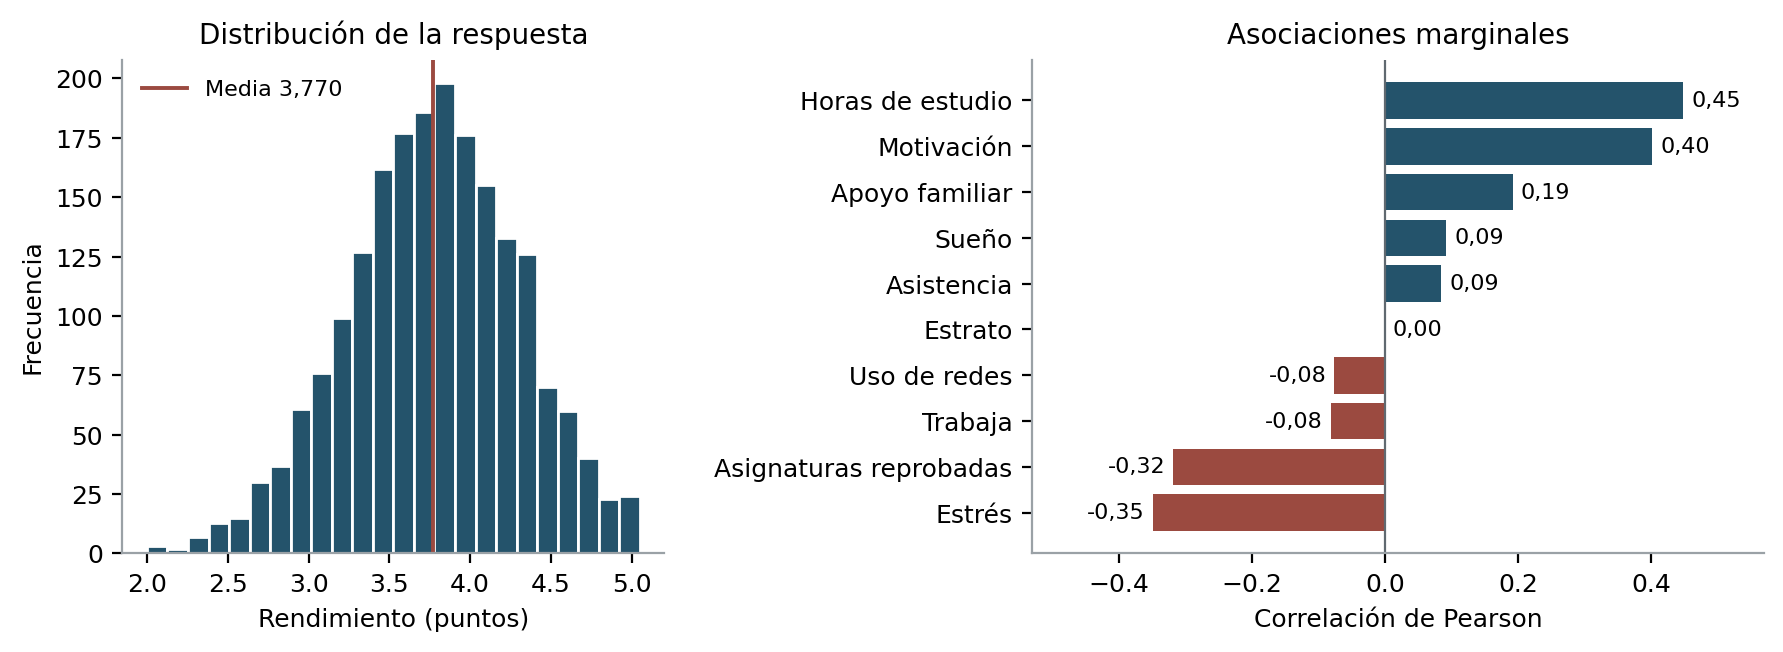
\includegraphics[width=1\textwidth,height=\textheight]{figuras/01_exploracion.png}
\caption{Figura 1. Distribución del rendimiento y correlaciones de
Pearson con los diez predictores. Las correlaciones son marginales y no
controlan las demás variables.}
\end{figure}

Las horas de estudio presentan la mayor correlación positiva con la nota
(\(r = 0{,}449\)), seguidas por la motivación (\(r = 0{,}402\)). El
estrés (\(r = -0{,}348\)) y las asignaturas reprobadas
(\(r = -0{,}318\)) muestran asociaciones negativas. El estrato tiene una
correlación cercana a cero. Estos valores describen pares de variables;
la interpretación parcial se obtiene con el modelo múltiple.

\newpage

\hypertarget{ajuste-del-modelo}{%
\subsection{4 Ajuste del modelo}\label{ajuste-del-modelo}}

La regresión lineal permite estudiar una respuesta cuantitativa mediante
varios predictores (James et al., 2013, cap. 3). Se estimó por mínimos
cuadrados ordinarios, sin interacciones ni selección automática. La
respuesta se mantiene en su escala de 0 a 5; las pruebas individuales
contrastan \(H_0:\beta_j=0\) con un nivel nominal de 0,05.

La ecuación estimada es:

\[
\begin{aligned}
\widehat{Y}={}&2{,}414689 + 0{,}048774H + 0{,}003978A + 0{,}198953M\\
 &-0{,}159582E + 0{,}102408F - 0{,}194610R - 0{,}086015T\\
 &+0{,}025021S - 0{,}028024U - 0{,}003527C.
\end{aligned}
\]

Aquí, \(H\) son horas de estudio; \(A\), asistencia; \(M\), motivación;
\(E\), estrés; \(F\), apoyo familiar; \(R\), asignaturas reprobadas;
\(T\), trabaja; \(S\), sueño; \(U\), uso de redes; y \(C\), estrato. La
ecuación describe la media condicional estimada. El modelo estadístico
incluye además un error \(\varepsilon_i\), con media condicional
supuesta igual a cero.

\textbf{Tabla 2. Coeficientes del modelo ajustado con las 2.000
observaciones.}

\begin{longtable}[]{@{}
  >{\raggedright\arraybackslash}p{(\columnwidth - 8\tabcolsep) * \real{0.2400}}
  >{\raggedleft\arraybackslash}p{(\columnwidth - 8\tabcolsep) * \real{0.1400}}
  >{\raggedleft\arraybackslash}p{(\columnwidth - 8\tabcolsep) * \real{0.1800}}
  >{\raggedleft\arraybackslash}p{(\columnwidth - 8\tabcolsep) * \real{0.3000}}
  >{\raggedleft\arraybackslash}p{(\columnwidth - 8\tabcolsep) * \real{0.1400}}@{}}
\toprule\noalign{}
\begin{minipage}[b]{\linewidth}\raggedright
Término
\end{minipage} & \begin{minipage}[b]{\linewidth}\raggedleft
Coeficiente
\end{minipage} & \begin{minipage}[b]{\linewidth}\raggedleft
Error estándar
\end{minipage} & \begin{minipage}[b]{\linewidth}\raggedleft
IC del 95 \%
\end{minipage} & \begin{minipage}[b]{\linewidth}\raggedleft
p
\end{minipage} \\
\midrule\noalign{}
\endhead
\bottomrule\noalign{}
\endlastfoot
Intercepto & 2,4147 & 0,0811 & {[}2,2555; 2,5738{]} & \textless{}
0,001 \\
Horas de estudio & 0,0488 & 0,0013 & {[}0,0461; 0,0514{]} & \textless{}
0,001 \\
Asistencia & 0,0040 & 0,0008 & {[}0,0025; 0,0055{]} & \textless{}
0,001 \\
Motivación & 0,1990 & 0,0058 & {[}0,1876; 0,2103{]} & \textless{}
0,001 \\
Estrés & -0,1596 & 0,0057 & {[}-0,1709; -0,1483{]} & \textless{}
0,001 \\
Apoyo familiar & 0,1024 & 0,0058 & {[}0,0911; 0,1137{]} & \textless{}
0,001 \\
Asignaturas reprobadas & -0,1946 & 0,0068 & {[}-0,2080; -0,1812{]} &
\textless{} 0,001 \\
Trabaja & -0,0860 & 0,0145 & {[}-0,1144; -0,0576{]} & \textless{}
0,001 \\
Sueño & 0,0250 & 0,0045 & {[}0,0162; 0,0338{]} & \textless{} 0,001 \\
Uso de redes & -0,0280 & 0,0044 & {[}-0,0367; -0,0194{]} & \textless{}
0,001 \\
Estrato & -0,0035 & 0,0050 & {[}-0,0134; 0,0063{]} & 0,4829 \\
\end{longtable}

\emph{Intervalos y errores estándar convencionales de mínimos cuadrados.
Los resultados se redondean para lectura; el código y los CSV conservan
mayor precisión.}

El coeficiente de determinación es \(R^2 = 0{,}6846\) y el ajustado es
\(0{,}6830\). Esto significa que el modelo recoge el \textbf{68,46 \% de
la variación de las notas dentro de esta base}. No significa que prediga
correctamente al 68,46 \% de los estudiantes. La desviación residual
estimada es de 0,2984 puntos.

La prueba global da \(F(10,1989)=431{,}67\), con \(p<0{,}001\). Se
rechaza que todas las pendientes sean simultáneamente cero. Ese
resultado indica que al menos un predictor aporta asociación lineal; no
demuestra que todos sean relevantes ni establece causalidad.

\newpage

\hypertarget{interpretaciuxf3n-de-los-coeficientes}{%
\subsection{5 Interpretación de los
coeficientes}\label{interpretaciuxf3n-de-los-coeficientes}}

Cada pendiente representa un cambio en el rendimiento esperado
\textbf{manteniendo constantes las demás variables del modelo}, como
indica la guía de coeficientes suministrada. Las unidades importan. Un
coeficiente pequeño puede corresponder a una variable medida en una
escala más amplia.

\textbf{Horas de estudio.} Una hora adicional se asocia con un aumento
de 0,0488 puntos en la nota. Para una diferencia de cinco horas, el
contraste estimado es de 0,244 puntos, con un intervalo de confianza del
95 \% entre 0,231 y 0,257. La interpretación conserva el período de
medición del archivo, que no especifica si se trata de horas semanales.

\textbf{Asistencia.} Un punto porcentual adicional se asocia con 0,00398
puntos más de rendimiento. Pasar de 80 \% a 90 \% equivale a diez puntos
porcentuales y representa un aumento estimado de 0,0398 puntos. En el
generador, el término es \texttt{0.03\ *\ asistencia\ /\ 10}: su
pendiente por punto porcentual es 0,003, no 0,03. La estimación recupera
una asociación pequeña y positiva.

\textbf{Motivación y apoyo familiar.} Un punto adicional en la escala de
motivación se asocia con 0,1990 puntos más de nota. Para el apoyo
familiar, la asociación por punto es de 0,1024. Ambos intervalos de
confianza quedan por encima de cero. Estas escalas se tratan como
cuantitativas por la estructura de la simulación; no se dispone de
información sobre un instrumento de medición validado.

\textbf{Estrés y asignaturas reprobadas.} Un punto adicional de estrés
se asocia con 0,1596 puntos menos de rendimiento. Una asignatura
reprobada adicional se relaciona con una disminución de 0,1946 puntos.
No se puede interpretar esta última relación como un efecto temporal sin
conocer cuándo se midieron las reprobaciones y la nota.

\textbf{Trabajo.} Los registros de personas que trabajan presentan una
nota esperada 0,0860 puntos menor que los de quienes no trabajan, bajo
control de los otros predictores. El intervalo del 95 \% va de −0,1144 a
−0,0576. Es una comparación entre las categorías 1 y 0; no mide el
efecto de una hora adicional de trabajo.

\textbf{Sueño y redes sociales.} Una hora adicional de sueño se asocia
con 0,0250 puntos más de rendimiento. Una hora diaria adicional de redes
se asocia con 0,0280 puntos menos. Son asociaciones de magnitud moderada
o pequeña en la escala de la nota, aunque sus valores p son inferiores a
0,001.

\textbf{Estrato.} La pendiente es −0,0035 y su intervalo del 95 \%
incluye cero: {[}−0,0134; 0,0063{]}. Con \(p=0{,}4829\), no hay
evidencia suficiente de una tendencia lineal parcial. Esto no prueba que
el contexto socioeconómico sea irrelevante en la vida real. En esta
simulación, el estrato no forma parte de la ecuación que genera el
rendimiento.

\textbf{Intercepto.} El valor 2,4147 corresponde a la predicción cuando
todos los predictores valen cero. Ese perfil queda fuera del soporte de
variables como asistencia y estrato. El intercepto es necesario para
ajustar el plano de regresión, pero no representa la nota de un
estudiante típico.

\newpage

\hypertarget{evaluaciuxf3n-de-los-supuestos}{%
\subsection{6 Evaluación de los
supuestos}\label{evaluaciuxf3n-de-los-supuestos}}

Los gráficos de residuos complementan las pruebas numéricas; la
normalidad se revisa sobre los errores aproximados por residuos, no
sobre cada predictor. Montgomery et al.~(2012, caps. 4, 6 y 9)
desarrollan el uso de estos diagnósticos y de las medidas de influencia
y colinealidad.

\textbf{Tabla 3. Diagnósticos del modelo principal.}

\begin{longtable}[]{@{}
  >{\raggedright\arraybackslash}p{(\columnwidth - 4\tabcolsep) * \real{0.2000}}
  >{\raggedright\arraybackslash}p{(\columnwidth - 4\tabcolsep) * \real{0.4000}}
  >{\raggedright\arraybackslash}p{(\columnwidth - 4\tabcolsep) * \real{0.4000}}@{}}
\toprule\noalign{}
\begin{minipage}[b]{\linewidth}\raggedright
Aspecto
\end{minipage} & \begin{minipage}[b]{\linewidth}\raggedright
Resultado
\end{minipage} & \begin{minipage}[b]{\linewidth}\raggedright
Lectura
\end{minipage} \\
\midrule\noalign{}
\endhead
\bottomrule\noalign{}
\endlastfoot
Forma funcional & RESET \(F(2,1987)=2{,}9946\); \(p=0{,}0503\) &
Resultado fronterizo. No se rechaza al 5 \%, pero requiere cautela. \\
Varianza residual & Breusch-Pagan studentizado: \(LM=6{,}8836\); 10 gl;
\(p=0{,}7364\) & No se detecta heterocedasticidad con esta prueba. \\
Normalidad & Shapiro-Wilk \(W=0{,}9985\); \(p=0{,}0830\) & No se rechaza
normalidad al 5 \%. No equivale a demostrarla. \\
Colinealidad & VIF entre 1,0012 y 1,0088 & No se observa inflación
importante de las varianzas. \\
Independencia & Simulación sin estructura temporal; Durbin-Watson =
2,0211 & El diseño respalda la independencia. El estadístico por orden
de fila es solo descriptivo. \\
\end{longtable}

\begin{figure}
\centering
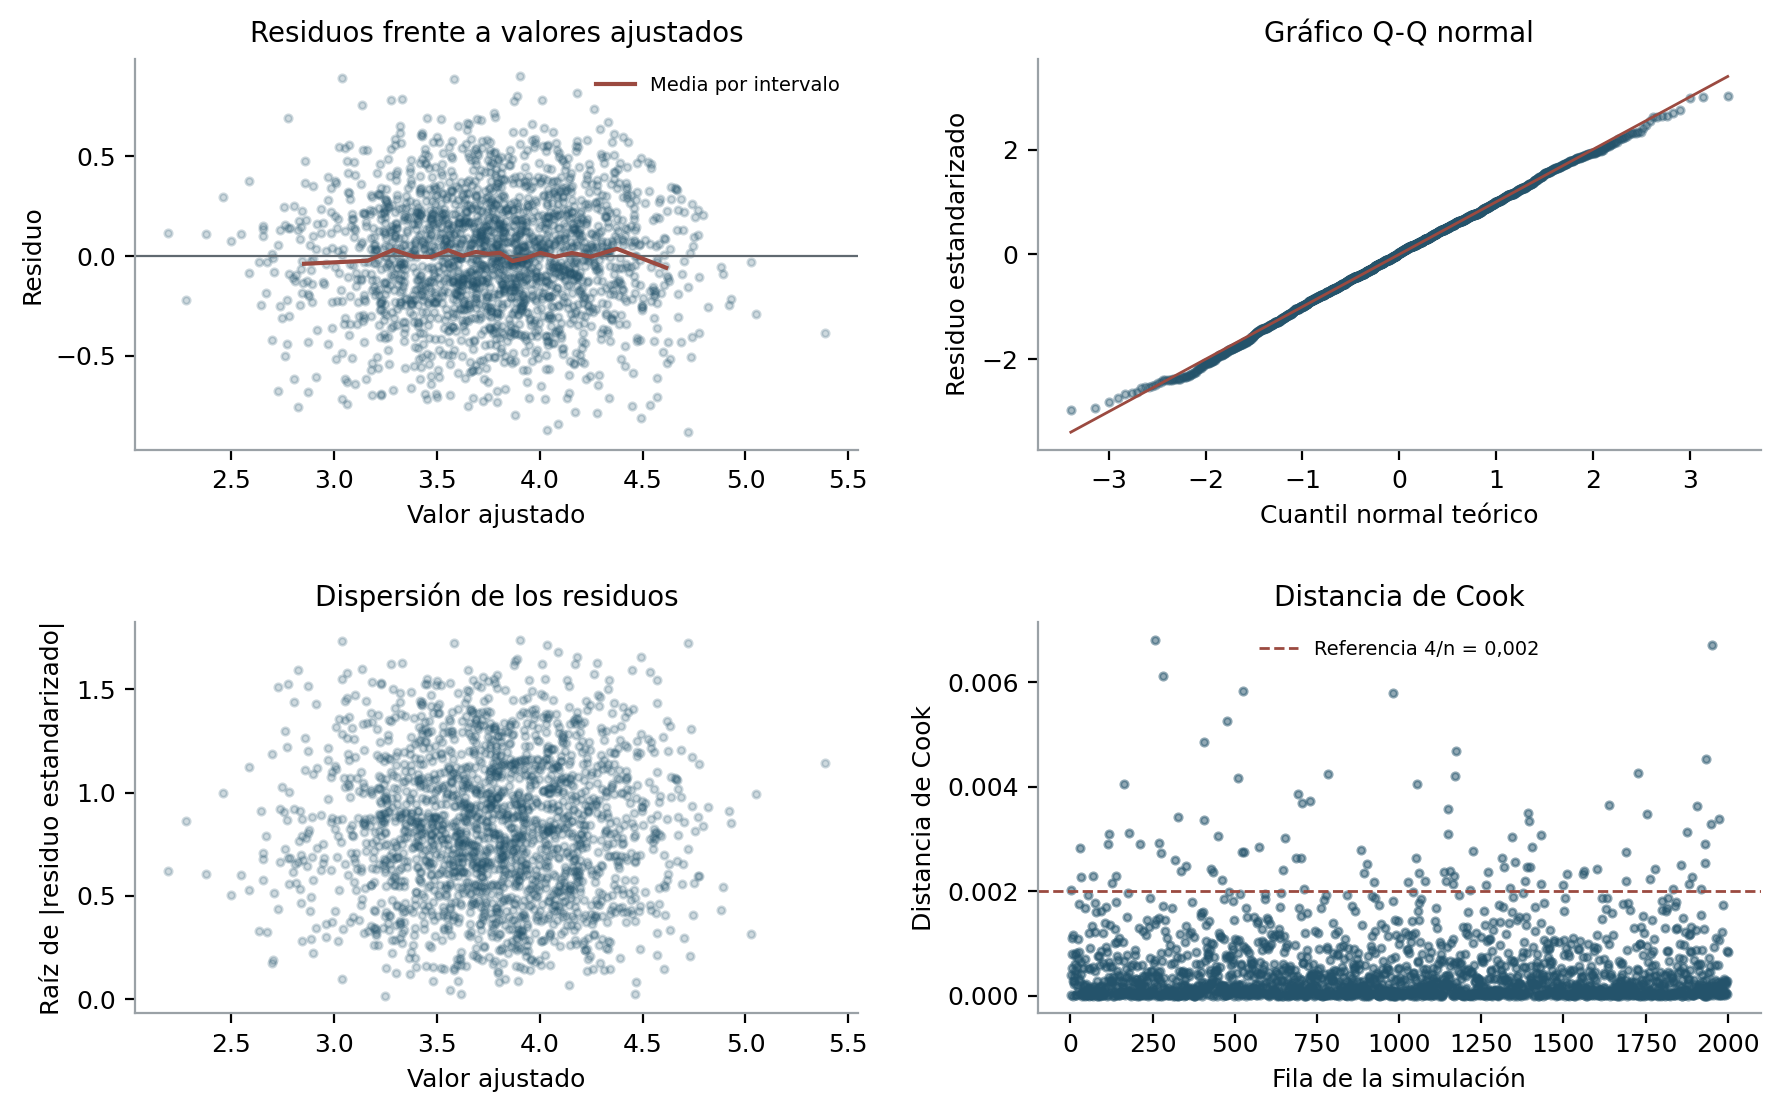
\includegraphics[width=1\textwidth,height=\textheight]{figuras/02_diagnosticos.png}
\caption{Figura 2. Diagnósticos del modelo con las 2.000 filas. La línea
roja del primer panel muestra medias de residuos por intervalos de
valores ajustados.}
\end{figure}

El gráfico Q-Q se aproxima a la recta y los residuos se centran cerca de
cero. El recorte de notas en 5 y el resultado fronterizo de RESET
justifican mantener reservas sobre la forma lineal.

\newpage

\hypertarget{influencia-y-anuxe1lisis-de-sensibilidad}{%
\subsection{7 Influencia y análisis de
sensibilidad}\label{influencia-y-anuxe1lisis-de-sensibilidad}}

La distancia de Cook máxima es 0,00681. Ninguna fila supera 1, pero 101
exceden la referencia \(4/n=0{,}002\). Ese umbral sirve para localizar
observaciones que conviene revisar, no como una orden de eliminación.
También hay 22 filas con apalancamiento superior a \(2p/n=0{,}011\),
donde \(p=11\) incluye el intercepto, y dos residuos studentizados
externos con valor absoluto mayor que 3.

Se mantuvieron todos los registros en el análisis principal. La tabla
siguiente permite comparar ese ajuste con dos escenarios de
sensibilidad: excluir las 56 filas con horas negativas y excluir, por
separado, las 101 alertas de Cook.

\textbf{Tabla 4. Estabilidad de las estimaciones bajo exclusiones de
sensibilidad.}

\begin{longtable}[]{@{}lrrr@{}}
\toprule\noalign{}
Término & Original & Sin horas negativas & Sin alertas de Cook \\
\midrule\noalign{}
\endhead
\bottomrule\noalign{}
\endlastfoot
Intercepto & 2,4147 & 2,4320 & 2,4732 \\
Horas de estudio & 0,0488 & 0,0483 & 0,0480 \\
Asistencia & 0,0040 & 0,0040 & 0,0036 \\
Motivación & 0,1990 & 0,1999 & 0,2004 \\
Estrés & -0,1596 & -0,1611 & -0,1632 \\
Apoyo familiar & 0,1024 & 0,1032 & 0,1004 \\
Asignaturas reprobadas & -0,1946 & -0,1943 & -0,1955 \\
Trabaja & -0,0860 & -0,0858 & -0,0783 \\
Sueño & 0,0250 & 0,0249 & 0,0246 \\
Uso de redes & -0,0280 & -0,0298 & -0,0275 \\
Estrato & -0,0035 & -0,0048 & -0,0038 \\
\end{longtable}

\emph{Tamaños de muestra: 2.000, 1.944 y 1.899, respectivamente. Son
ajustes distintos; las exclusiones no se acumulan.}

Al retirar las horas negativas, la mayor variación absoluta entre las
pendientes es de 0,0018, correspondiente al uso de redes. Los signos se
mantienen. Al retirar las alertas de Cook, la diferencia más alta entre
las pendientes es de 0,0078 para \texttt{trabaja}. La lectura sustantiva
permanece similar. El aumento de \(R^2\) al descartar observaciones
influyentes no debe presentarse como una mejora predictiva: se están
retirando casos en función del ajuste.

La inferencia con errores estándar robustos HC3 conserva las decisiones
al 5 \%: los nueve predictores distintos del estrato muestran evidencia
de asociación y el estrato sigue sin hacerlo. HC3 modifica la estimación
de incertidumbre, no los coeficientes ni la forma funcional del modelo.

También se comparó el tratamiento lineal del estrato con una
codificación mediante cinco indicadores, tomando una categoría como
referencia. Los cuatro parámetros adicionales no aportan evidencia de
mejora frente a la tendencia lineal: \(F=0{,}4577\) y \(p=0{,}7668\). Se
conserva la especificación del material. Esta comparación no convierte
las categorías ordinales en una escala métrica ni prueba que las seis
categorías tengan la misma media.

\newpage

\hypertarget{evaluaciuxf3n-predictiva}{%
\subsection{8 Evaluación predictiva}\label{evaluaciuxf3n-predictiva}}

Un buen ajuste en la muestra no basta para evaluar predicciones nuevas.
Se separaron aleatoriamente 1.600 registros para entrenamiento y 400
para prueba, con semilla 2026. La fórmula se fijó antes de esta
evaluación. El modelo entrenado con el 80 \% se utilizó para predecir el
20 \% restante, sin incorporar sus respuestas al ajuste.

El RMSE expresa la raíz del error cuadrático medio y penaliza más los
errores grandes. El MAE mide el error absoluto medio. Ambos se reportan
en puntos de la nota. El \(R^2\) de prueba se calcula respecto a la
media de las respuestas del conjunto de prueba.

\textbf{Tabla 5. Desempeño del modelo y comparación con una predicción
constante.}

\begin{longtable}[]{@{}lrrrr@{}}
\toprule\noalign{}
Evaluación & n & RMSE & MAE & \(R^2\) \\
\midrule\noalign{}
\endhead
\bottomrule\noalign{}
\endlastfoot
Entrenamiento & 1600 & 0,2964 & 0,2373 & 0,6807 \\
Prueba & 400 & 0,3041 & 0,2426 & 0,6917 \\
Media de entrenamiento en prueba & 400 & 0,5515 & 0,4343 & -0,0140 \\
\end{longtable}

La predicción de referencia asigna a todos los casos de prueba la nota
media del entrenamiento. El modelo reduce su RMSE de 0,5515 a 0,3041,
una disminución del \textbf{44,86 \%}. Su MAE de 0,2426 indica que la
diferencia absoluta entre predicción y observación promedia unas 0,24
unidades de nota. No significa que todos los errores sean menores que
esa cifra.

\begin{figure}
\centering
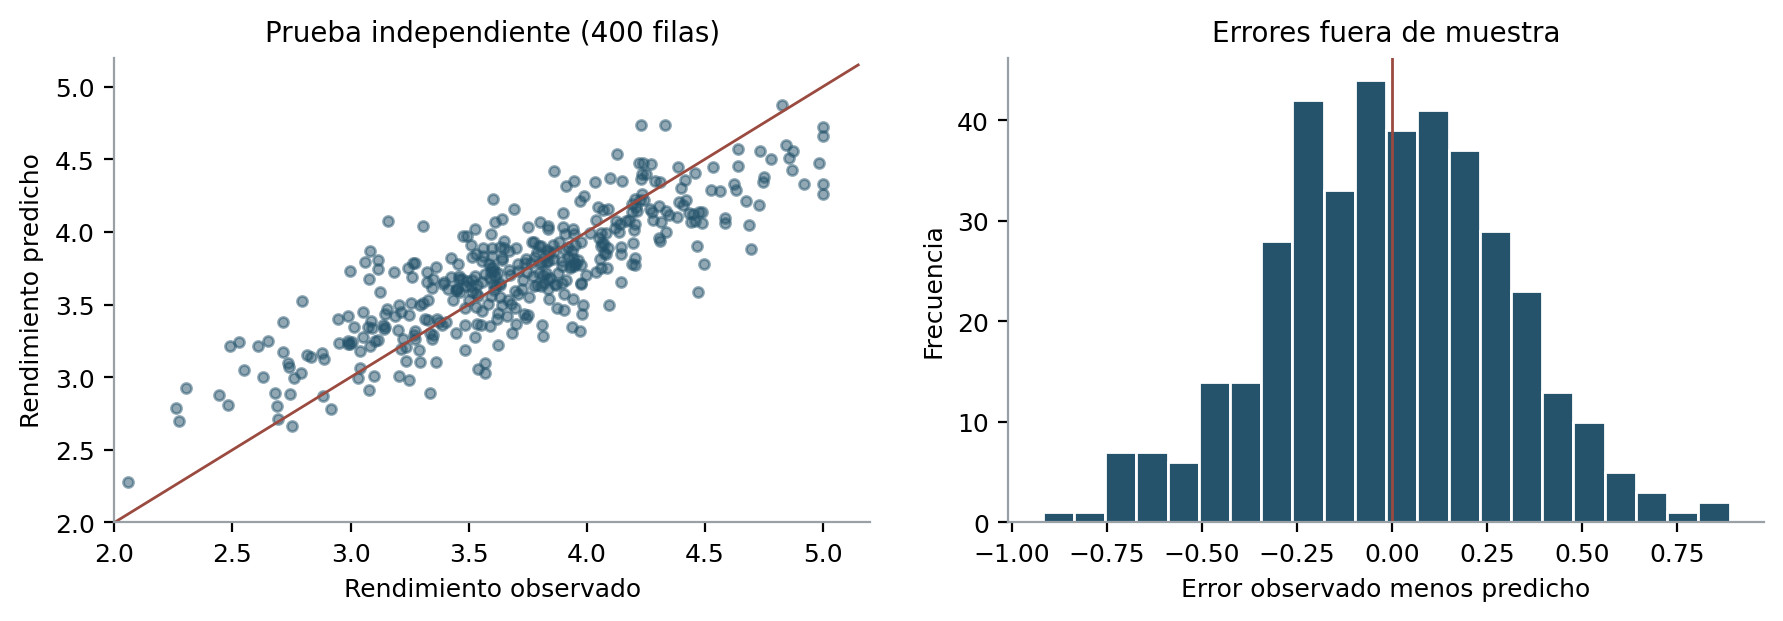
\includegraphics[width=1\textwidth,height=\textheight]{figuras/03_prediccion.png}
\caption{Figura 3. Predicciones y errores en los 400 registros
reservados para prueba. La diagonal indica predicción igual a
observación.}
\end{figure}

Como comprobación adicional, se realizó validación cruzada de cinco
particiones dentro del entrenamiento, con semilla 2027. El RMSE promedio
fue de 0,2985, con una desviación estándar entre particiones de 0,0071.
La cercanía con el resultado de prueba no sugiere un deterioro marcado
fuera de muestra en esta simulación; esa desviación no es un intervalo
de confianza.

Los intervalos de predicción nominales del 95 \% cubrieron 374 de los
400 valores observados, es decir, el 93,5 \%. Una predicción puntual
superó 5. La cobertura observada y el incumplimiento del límite de la
nota muestran por qué el error medio debe acompañarse de una revisión de
incertidumbre y rango.

\newpage

\hypertarget{ejemplo-de-predicciuxf3n-y-discusiuxf3n}{%
\subsection{9 Ejemplo de predicción y
discusión}\label{ejemplo-de-predicciuxf3n-y-discusiuxf3n}}

Una vez terminada la evaluación de prueba, se considera el modelo
ajustado con las 2.000 filas para ilustrar su uso. El perfil hipotético
tiene 15 horas de estudio, 90 \% de asistencia, motivación de 4, estrés
de 2, apoyo familiar de 4, ninguna asignatura reprobada, no trabaja, 8
horas de sueño, 2 horas diarias de redes y estrato 3. Es un ejemplo
construido para interpretar la ecuación, no una persona observada.

La predicción es de \textbf{4,524 puntos}. El intervalo de confianza del
95 \% para la media de perfiles con esas características es {[}4,491;
4,557{]}. El intervalo de predicción del 95 \% para un registro
individual es más amplio: {[}3,938; 5,110{]}. El primero describe
incertidumbre sobre la media; el segundo añade la variabilidad
individual contemplada por el modelo.

El límite superior de 5,110 es incompatible con la escala de
calificación. Se conserva tal como lo calcula el modelo para hacer
visible la limitación. Recortarlo a 5 y seguir llamándolo un intervalo
calibrado del 95 \% no resolvería el problema estadístico. Para una
aplicación real habría que evaluar un modelo que respete el límite,
reunir datos adecuados y comprobar su calibración.

\hypertarget{alcance-de-los-hallazgos}{%
\subsubsection{Alcance de los
hallazgos}\label{alcance-de-los-hallazgos}}

La ecuación generadora asigna asociaciones positivas a estudio,
asistencia, motivación, apoyo familiar y sueño; negativas a estrés,
reprobaciones, trabajo y redes. El modelo recupera esos signos. Era
razonable esperarlo, porque la simulación se construyó de esa manera. El
ejercicio demuestra que la estimación puede recuperar una estructura
conocida bajo ruido, pero no descubre qué determina el desempeño de
estudiantes reales.

Las variables psicosociales se generaron sin un instrumento validado y
varios predictores son independientes por construcción. Esto ayuda a
explicar los VIF próximos a uno, una situación que podría cambiar en una
base observacional. También faltan fechas y una población de referencia.
Sin temporalidad, diseño causal y control suficiente de factores
omitidos, no procede traducir las pendientes en efectos de una
intervención.

\hypertarget{conclusiones}{%
\subsection{10 Conclusiones}\label{conclusiones}}

\begin{enumerate}
\def\labelenumi{\arabic{enumi}.}
\tightlist
\item
  La regresión con los diez predictores del material explica el 68,46 \%
  de la variación del rendimiento simulado. La prueba global respalda
  una asociación conjunta, mientras que el estrato no muestra una
  tendencia lineal parcial claramente distinta de cero.
\item
  El modelo mantiene un desempeño parecido dentro y fuera del
  entrenamiento: obtiene un RMSE de 0,304 puntos en prueba y supera la
  predicción basada únicamente en la media. Esa utilidad predictiva
  queda restringida al mecanismo de simulación analizado.
\item
  Los diagnósticos no muestran colinealidad importante ni evidencia
  clara de heterocedasticidad. RESET queda cerca del umbral de decisión,
  por lo que la adecuación de la forma funcional requiere una lectura
  prudente.
\item
  Las horas negativas y las predicciones fuera de la escala deben
  documentarse. Las comprobaciones de sensibilidad sostienen las
  asociaciones principales, pero no sustituyen la revisión del generador
  ni habilitan recomendaciones sobre estudiantes reales.
\end{enumerate}

\newpage

\hypertarget{referencias}{%
\subsection{Referencias}\label{referencias}}

James, G., Witten, D., Hastie, T., y Tibshirani, R. (2013). \emph{An
introduction to statistical learning: With applications in R}. Springer.
Capítulo 3, pp.~59--126. https://doi.org/10.1007/978-1-4614-7138-7.
Recursos del libro: https://www.statlearning.com/

Montgomery, D. C., Peck, E. A., y Vining, G. G. (2012).
\emph{Introduction to linear regression analysis} (5.ª ed.). Wiley.
Capítulos 3, 4, 6, 9 y 11.
\href{https://www.kwcsangli.in/uploads/3--Introduction_to_Linear_Regression_Analysis__5th_ed._Douglas_C._Montgomery__Elizabeth_A._Peck__and_G._.pdf}{PDF
suministrado en la actividad}.

R Core Team. (s. f.). \emph{Fitting linear models} {[}Documentación de
\texttt{lm}{]}.
https://stat.ethz.ch/R-manual/R-devel/library/stats/html/lm.html

R Core Team. (s. f.). \emph{Predict method for linear model fits}
{[}Documentación de \texttt{predict.lm}{]}.
https://stat.ethz.ch/R-manual/R-devel/library/stats/html/predict.lm.html

R Core Team. (s. f.). \emph{Random number generation} {[}Documentación
de \texttt{RNGkind} y \texttt{set.seed}{]}.
https://stat.ethz.ch/R-manual/R-devel/library/base/html/Random.html

\emph{Dataset\_RegMultiple.R}. (s. f.). {[}Script suministrado en la
actividad{]}. Material de clase sin autor identificado en el archivo.

\emph{Guía Interpretación coeficientes}. (s. f.). {[}Presentación de
diapositivas suministrada en la actividad{]}. Material de clase sin
autor identificado en el archivo.

\emph{dataset\_RegMultiple.xlsx}. (s. f.). {[}Archivo suministrado en la
actividad{]}. Se revisó para contrastar su contenido con el generador;
no se utilizó para estimar el modelo.

\hypertarget{reproducciuxf3n-del-anuxe1lisis}{%
\subsubsection{Reproducción del
análisis}\label{reproducciuxf3n-del-anuxe1lisis}}

El archivo \texttt{analisis\_regresion\_multiple.R} reconstruye la base,
calcula el modelo y exporta tablas de coeficientes, intervalos,
diagnósticos por fila, particiones y predicciones. Utiliza funciones
incluidas en R y no necesita instalar paquetes adicionales. La base
entregada es \texttt{datos\_simulados\_R.csv}. La sesión de referencia
corresponde a R 4.3.3.

Desde la carpeta del trabajo se ejecuta:

\begin{Shaded}
\begin{Highlighting}[]
\ExtensionTok{Rscript}\NormalTok{ analisis\_regresion\_multiple.R}
\end{Highlighting}
\end{Shaded}

El script complementario \texttt{generar\_informe.py} crea las figuras y
las versiones Markdown, LaTeX, PDF y HTML a partir de las tablas. Sus
dependencias están en \texttt{requirements.txt}; la compilación requiere
Pandoc y XeLaTeX. El código fuente del informe y las figuras se incluyen
para permitir la revisión de la presentación.

La matriz de mínimos cuadrados se contrastó mediante un cálculo
independiente en Python; las diferencias frente a R fueron inferiores a
\(10^{-12}\). La base exportada también se comparó con la ejecución del
generador original, corrigiendo únicamente su llamada de exportación.
Las cifras de este documento proceden de esos cálculos, no de valores
inventados para ilustrar resultados.

\newpage

\hypertarget{anexo-de-uso-de-inteligencia-artificial}{%
\subsection{Anexo de uso de inteligencia
artificial}\label{anexo-de-uso-de-inteligencia-artificial}}

\hypertarget{propuxf3sito-y-alcance}{%
\subsubsection{Propósito y alcance}\label{propuxf3sito-y-alcance}}

Se utilizó ChatGPT, de OpenAI, para reproducir el ejercicio y comparar
un proceso ya desarrollado, con un rol de \textbf{revisor técnico
(viewer) y corrector ortográfico y de redacción}. La revisión tomó como
referencia el material de clase, el código y la primera versión del
informe. Durante su preparación, la herramienta también apoyó la
adaptación y ejecución del código, la elaboración de gráficos y la
redacción de las interpretaciones.

\hypertarget{solicitud-de-reproducciuxf3n-y-comparaciuxf3n}{%
\subsubsection{Solicitud de reproducción y
comparación}\label{solicitud-de-reproducciuxf3n-y-comparaciuxf3n}}

Para revisar esta versión, la petición se reformuló así:

\begin{quote}
Actúa como revisor técnico (viewer) y corrector ortográfico de un
ejercicio de regresión lineal múltiple ya desarrollado. Reproduce el
procedimiento y compara sus coeficientes, medidas de ajuste,
diagnósticos y predicciones con los resultados existentes.

Identifica instrucciones que funcionen en el entorno actual, pero puedan
fallar o producir resultados distintos en otras condiciones. Explica la
causa y sugiere cambios justificados. Revisa las interpretaciones y
corrige ortografía, puntuación y concordancia, conservando el sentido
del texto y las cifras verificadas.
\end{quote}

\hypertarget{sugerencias-realizadas-sobre-el-cuxf3digo}{%
\subsubsection{Sugerencias realizadas sobre el
código}\label{sugerencias-realizadas-sobre-el-cuxf3digo}}

\textbf{Reproducibilidad de la simulación.} El uso de
\texttt{set.seed(123)} es válido y permite repetir los datos bajo la
misma configuración. Sin embargo, la semilla por sí sola no fija los
algoritmos aleatorios activos. Si estos cambian entre sesiones o
versiones de R, la misma semilla puede producir otra secuencia. La
documentación de R registra, por ejemplo, un cambio en el algoritmo
predeterminado de \texttt{sample()} a partir de la versión 3.6.0 (R Core
Team, s. f., \emph{Random number generation}).

Se sugirió hacer explícita la configuración antes de fijar la semilla:

\begin{Shaded}
\begin{Highlighting}[]
\FunctionTok{RNGkind}\NormalTok{(}\StringTok{"Mersenne{-}Twister"}\NormalTok{, }\StringTok{"Inversion"}\NormalTok{, }\StringTok{"Rejection"}\NormalTok{)}
\FunctionTok{set.seed}\NormalTok{(}\DecValTok{123}\NormalTok{)}
\end{Highlighting}
\end{Shaded}

Este ajuste conserva el método de regresión y evita depender de una
configuración implícita. La versión entregada ya lo incorpora. También
se documentó R 4.3.3 como entorno de referencia y se mantuvo el orden de
las operaciones.

\textbf{Referencia al objeto exportado.} El archivo original construye
\texttt{datos}, pero intenta exportar \texttt{dataset}. Esa instrucción
podría escribir la base correcta si \texttt{dataset} existiera
previamente y contuviera los mismos datos. En una sesión limpia
fallaría; si contuviera otra base, exportaría información equivocada. Se
sugirió usar explícitamente el objeto creado por el script. Para
conservar Excel, la corrección sería:

\begin{Shaded}
\begin{Highlighting}[]
\FunctionTok{write.xlsx}\NormalTok{(datos, }\StringTok{"dataset\_RegMultiple.xlsx"}\NormalTok{)}
\end{Highlighting}
\end{Shaded}

La versión entregada utiliza \texttt{write.csv(datos,\ ...)}, con el
mismo criterio y sin requerir el paquete de exportación a Excel.

\hypertarget{comprobaciuxf3n-de-las-sugerencias}{%
\subsubsection{Comprobación de las
sugerencias}\label{comprobaciuxf3n-de-las-sugerencias}}

La configuración explícita reprodujo la base entregada. Una prueba con
otro algoritmo de muestreo y la misma semilla produjo diferencias en la
base, confirmando el riesgo señalado. Los coeficientes y errores
estándar se contrastaron entre R y Python, con diferencias inferiores a
\(10^{-12}\). Las sugerencias y la revisión lingüística conservaron las
cifras del informe.

\end{document}
